\section{Background}

%Background (10- 20 pages).  This should form the bulk of the interim report. You should consider that your objective here is to produce a near final version of the background section, as it will appear in your final report.  All of this material should be re-usable, so it is worth getting it right at this stage of the project.  The details of what to include can be found in the Project Report guidelines.

%The background section of the report should set the project into context by relating it to existing published work which you read at the start of the project when your approach and methods were being considered. There are usually many ways of solving a given problem, and you shouldn't just pick one at random. Describe and evaluate as many alternative approaches as possible. The published work may be in the form of research papers, articles, text books, technical manuals, or even existing software or hardware of which you have had hands-on experience. Your must acknowledge the sources of your inspiration. You are expected to have seen and thought about other people's ideas; your contribution will be putting them into practice in some other context. However, avoid plagiarism: if you take another person's work as your own and do not cite your sources of information/inspiration you are being dishonest; in other words you are cheating. When referring to other pieces of work, cite the sources where they are referred to or used, rather than just listing them at the end. Make sure you read and digest the Department's plagiarism document .

%In writing the Background chapter you must demonstrate your capability of analysis, synthesis and critical judgement. Analysis is shown by explaining how the proposed solution operates in your own words as well as its benefits and consequences. Synthesis is shown through the organisation of your Related Work section and through identifying and generalising common aspects across different solutions. Critical judgement is shown by discussing the limitations of the solutions proposed both in terms of their disadvantages and limits of applicability.

\subsection{A Stereo Approach}

A large amount of research has been done in the use of stereo cameras and 3D sensors for skeletal tracking. Much of this arose from the introduction of Microsoft's Kinect\cite{kinect} sensor which brought affordable and reliable depth perception to the general public.

\subsubsection{Kinect}

Jamie Shotton et al developed an algorithm\cite{shottonkinect} for human pose detection (that is the three-dimensional positions of body joints) which uses a Randomised Decision Forest trained on an extremely large data set of a wide variety of poses. This machine learning approach is used in the Kinect tracking system, and has the advantage of being both robust and computationally inexpensive to classify a new image. This is due to the algorithm reducing the detection into a per-pixel classification problem. Another advantage of this method is that it does not rely on temporal information (or previous frames) as pose estimation can be performed on a standalone frame.

However this machine learning approach may not be feasible in the scope of this project. There is not enough time available to collect the data required to train a machine learner such as this to recognise body pose. Shotton's results showed that in order to effectively detect a human pose, his system required training on at least 100,000 images\cite{shottonkinect}.
\subsubsection{Captury}

A company known as Captury\cite{captury} have constructed a method for robust motion capture using a stereo camera. In their paper `On-set Performance Capture of Multiple Actors With A Stereo Camera'\cite{capturystereopaper} they describe a method that ``employs appearance cues, scene flow, pose reconstruction results from previous frames, and stereo coherence to reliably segment out actors in front of general backgrounds.''. This method has been shown to be highly robust, and Captury have provided a video\cite{capturyvideo} to demonstrate this. Not only does their method track the skeleton, it also performs a further step to map a full three dimensional body to the video, for full motion capture.

Although immensely accurate, Captury's process requires a large amount of computation, in the order of minutes per frame. This means that use of an algorithm following their pipeline would not be able to achieve real-time feedback.

\subsubsection{Applied to this Project}

Unfortunately, despite the wide array of tools and libraries available for skeletal tracking with a 3D sensor or stereo camera, it would be infeasible to take a device like a Kinect hooked up to a computer into a gym. Perhaps if the goal were to have the system set up at powerlifting competitions, or pre-installed at gyms, this method would be more reasonable. However as a personal training aid, the device must be portable.

Another alternative option would be to develop an application for a smartphone with a stereo camera. Smartphones such as the LG Optimus 3D\cite{lgoptimus} provide such a camera. However these phones are not currently in wide use and would severely narrow the audience for this application.

For these reasons it has been chosen to employ a monocular approach. This will make foreground segmentation more challenging and so it has been decided to narrow the scope of the project to a known camera angle.


\section{Human Models}

A key part of my project will be the creation of a reliable human model to map to each frame, so that it mimics the pose of the lifter. In this section potential model options for use in this project will be considered.

\subsubsection{A Cardboard Model}

A possible representation is a so called ``carboard model'', which is a set of interconnected planar patches used to represent human limbs. This is used in `Cardboard People: A Parameterized Model of Articulated Image Motion'\cite{cardboardpeople}, where S. Ju et al tracked a walking movement in two dimensions using two body parts - the thigh and the calf. These articulated components were governed by their `translation' and `curl' (that is rotation) in a side view of the walk. For more robust modelling from other camera angles, components could be governed by their `divergence', `deformation', `yaw' and `pitch'. The culmination of these parameters defines each cardboard segment's location in two-dimensional space, but compensates for three-dimensional movement of the subject. Figure~\ref{fig:cardboardmodel} shows an example model and the effects of adjustments of these parameters.

\begin{figure}[H]
    \centering
    \subfigure[A cardboard model]{
            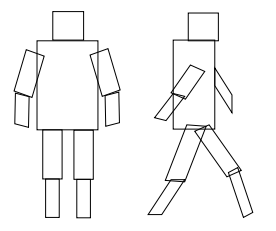
\includegraphics[height=6cm]{background/images/cardboard}
    }
    \subfigure[Parameters governing position of a cardboard segment]{
            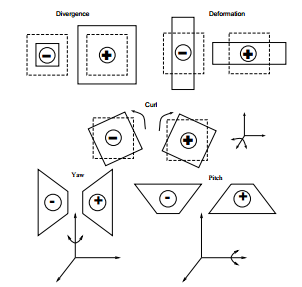
\includegraphics[height=6cm]{background/images/cardboard2}
    }
\caption{The cardboard model used by S. Ju et al\cite{cardboardpeople}}
\label{fig:cardboardmodel}
\end{figure}

Other similar primitive shape representations such as cylinders, ellipsoids and cones are often used\cite{cvmocapsurvey}.
\subsubsection{Stick Figure Model}

Motion capture of human walking has been carried out in `Lower Limb Kinematics of Human Walking with the Medial Axis Transformation'\cite{stickfigure}, where instead of a fleshed out model like the cardboard model, A. Bharatkumar et al used a stick figure to represent the human body. In this paper they concluded that ``It is easier to track the segment angles of the thigh and leg than the actual positions of the joints''. This makes mapping much simpler than that of the cardboard model, as there are far fewer parameters to optimise. Although they did not add explicit constraints to the model in their paper, it would be easy to add such constraints to ensure a better fit of the model to the frame. Figure~\ref{fig:stickfiguremodel} shows a full three-dimensional stick figure model, and a two-dimensional model of the thigh and calf.

\begin{figure}[H]
    \centering
    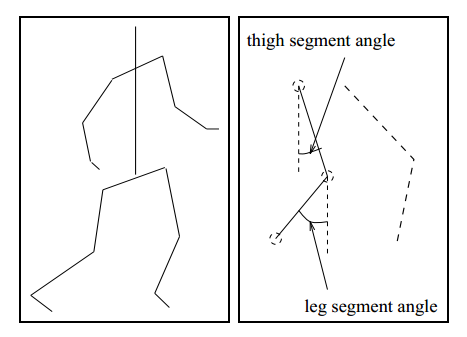
\includegraphics[height=6cm]{background/images/stickfigure}

	\caption{The stick figure model used by A. Bharatkumar et al\cite{stickfigure}}
	\label{fig:stickfiguremodel}
\end{figure}
\subsubsection{A Three-Dimensional Model}

As well as models constructed from primitive two-dimensional shapes, we can extend these models into three dimensions. Some solutions are simple expansions of these primitives into their three-dimensional counter parts, but others are more intricate. M. Yamamoto et al used Computer Aided Design to develop a model constructed of conical cylinders and cuboids\cite{cadmodel}. Another example of this is shown in Figure~\ref{fig:3dmodelajd} where a range of three-dimensional shapes are mapped to a human figure by J. Deutscher et al.

\begin{figure}[H]
    \centering
    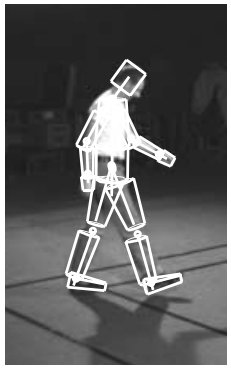
\includegraphics[height=6cm]{background/images/3dpolygon}

	\caption{A model constructed of three-dimensional primitive shapes\cite{stickfigure}}
	\label{fig:3dmodelajd}
\end{figure}

Some have used more advanced techniques to construct a customised model to be used to track a known person. C. Wu et al performed a three-dimensional scan of the subjects to generate a textured model of each person to be tracked\cite{capturystereopaper}. Several others have used similar techniques, creating a more `life like' model of a human. This has advantages in being able to fit the subject more accurately, but requires an additional step to create the model of a new subject prior to tracking them. Figure~\ref{fig:3dtexturedmodel} shows an example of a model generated in this way and mapped to a frame of video.

\begin{figure}[H]
    \centering
    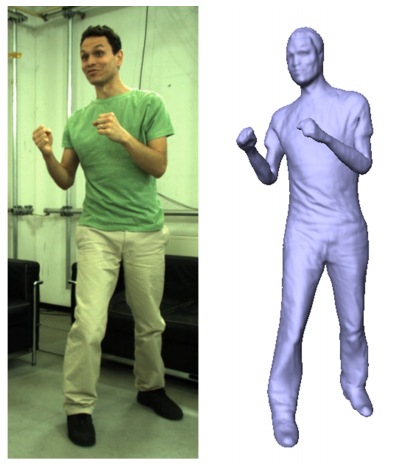
\includegraphics[height=6cm]{background/images/3dtexture}

	\caption{A more advanced model, specific to an individual subject\cite{capturystereopaper}}
	\label{fig:3dtexturedmodel}
\end{figure}
\subsubsection{Applied to this Project}

This project will be using a monocular camera. This does not necessarily mean that the mapping of a three dimensional model to a two dimensional frame is not impossible, but is more computationally challenging. In the case of squatting, we can extract all required data to determine the validity of a lift from a two dimensional model of the side view. The only information that we would miss with a two dimensional model is one related to the safety of the lifts: the position of the knees from a front view, to make sure that they do not buckle in towards each other. This is an acceptable compromise, being only a single measure out of many.

The camera will be in a known location relative to the human subject and the movements are well defined, which makes a two dimensional model feasible. As it will provide us with enough data to determine the validity and to measure the majority of safety criteria of the lift, I have opted to use a two dimensional model for this project.

This two dimensional model will likely be based on the cardboard model, using two dimensional shapes that best fit the human subject. Their positions should not individually be defined by their position, rotation, yaw etc, but should be defined by the relative rotations at joints. This will reduce the degrees of freedom of the model, allowing for faster optimisation. It will also more accurately represent a human and the human limits of joint movement can be used to constrain the optimisation problem.

\subsection{Foreground Segmentation}

We must separate the lifter from their surroundings in order to provide a silhouette to map our human model to.

\subsubsection{Background Subtraction}

The background subtraction in general is to compute the per pixel differences between a given frame and a known background frame. Differences above a certain threshold are considered foreground, and differences below this threshold are considered background.

The background image is often obtained from either a frame from the video sequence known to be background, or by taking the average pixel values over a selection (or all) frames in a video sequence.

More advanced implementations of background subtraction will use mixtures of gaussians to represent colours in the frame, with each gaussian weighted by the time that colour remains in the scene\cite{backgroundsubmog}. Colours considered to be background are those that stay in the scene longer, with less motion. Implementations such as this are used in OpenCV\cite{opencv}.
%\input{background/foregroundsegmentation/}

\subsection{Fitting a Model to a Frame}